% =====================================================================
%  COMP 333 Project -- Phase 2 Report
%  Unified 2D Shape Classifier
%  Built by the pipeline:  .\build.ps1 -File phase2_report.tex
%  (Stage 6, src/stage6_report/run.py; the -File argument is mandatory)
%
%  Traceability rule (stages/stage_6.md): every number about data or
%  results comes from an artifact through \InputIfFileExists or a generated
%  macro. Nothing quantitative is typed by hand in this file; plan constants
%  (70/15/15, 64x64, 10 classes) are the only bare numbers allowed, and
%  src/stage6_report/traceability.py checks that at build time.
% =====================================================================
\documentclass[11pt]{article}
\usepackage[margin=0.5in]{geometry}
\usepackage{amsmath}
\usepackage{booktabs}
\usepackage{tabularx}
\usepackage{array}
\usepackage{float}
\usepackage{caption}
\usepackage{xcolor}
\usepackage{graphicx}
\usepackage{tikz}
\usetikzlibrary{positioning,arrows.meta,calc,shapes.geometric}
\usepackage[colorlinks=true, linkcolor=blue, citecolor=blue,
            urlcolor=blue]{hyperref}  % links, refs and citations in blue

% ---------------------------------------------------------------------
% Generated inputs. Each file is optional: the report always compiles, and
% a missing artifact shows as "--" (the Stage 6 status lists it as missing).
% ---------------------------------------------------------------------
% Stage 1: split counts, gemstone state, near-duplicate groups.
\InputIfFileExists{artifacts/stage1/report_counts.tex}{}{}
\providecommand{\SplitTrain}{--}
\providecommand{\SplitVal}{--}
\providecommand{\SplitTest}{--}
\providecommand{\SplitTotal}{--}
\providecommand{\GemstonesRemoved}{--}
\providecommand{\GemstoneFilterState}{not yet applied (review pending)}
\providecommand{\NearDupGroups}{--}
\providecommand{\LargestNearDupGroup}{--}
% Stage 6: facts from the Stage 1/3/4/5 status files, the config and export/.
% Sections A to J report iteration 1 from frozen copies, so later runs cannot change them.
\InputIfFileExists{docs/crisp_dm/iteration_1/pipeline_facts.tex}{}{}
\InputIfFileExists{artifacts/stage6/generated/iteration2_facts.tex}{}{}
% CRISP-DM iteration 1: committed evidence (validation only) + Stage 1 count.
\InputIfFileExists{docs/crisp_dm/iteration_1_quickdraw_diamonds.tex}{}{}
\InputIfFileExists{artifacts/stage1/exclusions.tex}{}{}
\providecommand{\ExcludedByRule}{--}
\providecommand{\IterOneAZeroSeedZeroMacroFone}{--}
\providecommand{\IterOneAZeroSeedZeroDiamondFone}{--}
\providecommand{\IterOneAZeroSeedZeroQDRecall}{--}
\providecommand{\IterOneAZeroSeedZeroRenderRecall}{--}
\providecommand{\IterOneAZeroSeedZeroQDAsTriangle}{--}
\providecommand{\IterOneAZeroSeedZeroQDN}{--}
\providecommand{\IterOneAZeroSeedTwoMacroFone}{--}
\providecommand{\IterOneAZeroSeedTwoDiamondFone}{--}
\providecommand{\IterOneAZeroSeedTwoQDRecall}{--}
\providecommand{\IterOneAZeroSeedTwoRenderRecall}{--}
\providecommand{\IterOneAZeroSeedTwoQDAsTriangle}{--}
\providecommand{\IterOneAOneSeedZeroMacroFone}{--}
\providecommand{\IterOneAOneSeedZeroDiamondFone}{--}
\providecommand{\IterOneAOneSeedZeroQDRecall}{--}
\providecommand{\IterOneAOneSeedZeroRenderRecall}{--}
\providecommand{\IterOneAOneSeedZeroQDAsTriangle}{--}
\providecommand{\IterOneAOneSeedTwoMacroFone}{--}
\providecommand{\IterOneAOneSeedTwoDiamondFone}{--}
\providecommand{\IterOneAOneSeedTwoQDRecall}{--}
\providecommand{\IterOneAOneSeedTwoRenderRecall}{--}
\providecommand{\IterOneAOneSeedTwoQDAsTriangle}{--}
\providecommand{\ItwoPrimary}{--}
\providecommand{\ItwoDelta}{--}
\providecommand{\ItwoCILo}{--}
\providecommand{\ItwoCIHi}{--}
\providecommand{\ItwoVerdict}{--}
\providecommand{\ItwoReads}{--}
\providecommand{\ItwoFreshN}{--}
\providecommand{\ItwoFreshDelta}{--}
\providecommand{\ItwoFreshCILo}{--}
\providecommand{\ItwoFreshCIHi}{--}
\providecommand{\ItwoFreshVerdict}{--}
\providecommand{\ItwoRotate}{--}
\providecommand{\ItwoRotateCap}{--}
\providecommand{\ItwoAtwoClean}{--}
\providecommand{\ItwoAtwoSynth}{--}
\providecommand{\ItwoBSynth}{--}
\providecommand{\ItwoEnsAzero}{--}
\providecommand{\ItwoEnsAone}{--}
\providecommand{\ItwoEnsB}{--}
\providecommand{\ItwoEnsAtwo}{--}
\providecommand{\ItwoFreshAzero}{--}
\providecommand{\ItwoFreshAone}{--}
\providecommand{\ItwoFreshB}{--}
\providecommand{\ItwoFreshAtwo}{--}
\providecommand{\ItwoValAzero}{--}
\providecommand{\ItwoValAone}{--}
\providecommand{\ItwoValB}{--}
\providecommand{\ItwoValAtwo}{--}
\providecommand{\ItwoTrialsAzero}{--}
\providecommand{\ItwoTrialsAone}{--}
\providecommand{\ItwoTrialsB}{--}
\providecommand{\ItwoTrialsAtwo}{--}
\providecommand{\ItwoLosoAzero}{--}
\providecommand{\ItwoLosoAone}{--}
\providecommand{\ItwoLosoB}{--}
\providecommand{\ItwoLosoAtwo}{--}
\providecommand{\BatchSize}{--}
\providecommand{\SeedsPerArm}{--}
\providecommand{\SyntheticSharePct}{--}
\providecommand{\MaxEpochs}{--}
\providecommand{\Patience}{--}
\providecommand{\TuningArm}{--}
\providecommand{\TuningLRs}{--}
\providecommand{\TuningDropouts}{--}
\providecommand{\Alpha}{--}
\providecommand{\NBoot}{--}
\providecommand{\MinGainPoints}{--}
\providecommand{\MaxClassDropPoints}{--}
\providecommand{\CILevelPct}{--}
\providecommand{\PhashHammingMax}{--}
\providecommand{\SplitRatios}{--}
\providecommand{\ImageSize}{--}
\providecommand{\NumClasses}{--}
\providecommand{\NumRuns}{--}
\providecommand{\PowerLimitPoints}{--}
\providecommand{\ShortcutTriggerPoints}{--}
\providecommand{\GemstoneFilterSetting}{--}
\providecommand{\ShortcutDetected}{--}
\providecommand{\SourceGainPoints}{--}
\providecommand{\SourceClassifierAccPct}{--}
\providecommand{\SourceMajorityRatePct}{--}
\providecommand{\ThroughputSynth}{--}
\providecommand{\ThroughputTarget}{--}
\providecommand{\StepsPerEpoch}{--}
\providecommand{\TunedLR}{--}
\providecommand{\TunedDropout}{--}
\providecommand{\RealDrawsA}{--}
\providecommand{\RealDrawsB}{--}
\providecommand{\SynthDrawsB}{--}
\providecommand{\LoaderImagesPerSec}{--}
\providecommand{\SeedDisagreementAzero}{--}
\providecommand{\SeedDisagreementAone}{--}
\providecommand{\SeedDisagreementB}{--}
\providecommand{\LosoRequired}{--}
\providecommand{\LosoHoldoutSource}{--}
\providecommand{\Verdict}{--}
\providecommand{\TestReads}{--}
\providecommand{\RunId}{--}
\providecommand{\ExportedRun}{--}
\providecommand{\ExportedArm}{--}
\providecommand{\ExportedValFone}{--}

% Guarded figure: shows the image when the artifact exists, a labelled box otherwise.
\newcommand{\MissingFigure}[2]{\fbox{\parbox[c][2.5cm][c]{\dimexpr#1-2\fboxsep-2\fboxrule\relax}{\centering\footnotesize not generated yet:\\ \nolinkurl{#2}}}}
\newcommand{\GuardedGraphic}[2]{\IfFileExists{#2}{\includegraphics[width=#1]{#2}}{\MissingFigure{#1}{#2}}}

\newcommand{\TBD}{\textcolor{red}{\textbf{TBD}}}
\newcommand{\pending}{\textcolor{red}{pending: official rubric not yet supplied}}

\captionsetup{font=small,labelfont=bf}
\setlength{\emergencystretch}{2em}  % let long file names wrap cleanly

% Border around every page, 0.3in in from the paper edge (text margin is 0.5in)
\AddToHook{shipout/background}{%
  \begin{tikzpicture}[remember picture, overlay]
    \draw[line width=0.8pt]
      ($(current page.north west)+(0.3in,-0.3in)$) rectangle
      ($(current page.south east)+(-0.3in,0.3in)$);
  \end{tikzpicture}}

\title{Unified 2D Shape Classifier\\[4pt]
       \large COMP 333 -- Phase 2 Report}
\author{}
\date{\today}

\begin{document}
\maketitle

\begin{center}
\IfFileExists{figures/cover_banner.png}{
\includegraphics[width=0.9\linewidth]{figures/cover_banner.png}\\[2pt]
{\scriptsize\color{gray} Cover art: roszie, Pixabay
(\url{https://pixabay.com/illustrations/geometric-art-colorful-shapes-7409280/})}}{}
\end{center}

\begin{table}[H]
\centering
\caption{Team members.}
\begin{tabular}{@{}lr@{}}
\toprule
Name & Student ID \\
\midrule
Yahya Belgharbi         & \TBD \\
Fiacre Byiringiro       & \TBD \\
Damiano Confuorti       & \TBD \\
Jananaa Mahathevan      & \TBD \\
Yash Dilipkumar Nathani & \TBD \\
Ray Ntukanyagwe         & \TBD \\
\bottomrule
\end{tabular}
\end{table}

\begin{center}
\setlength{\fboxsep}{10pt}
\fbox{\begin{minipage}{0.92\linewidth}
\tableofcontents
\end{minipage}}
\end{center}
\newpage

% =====================================================================
\section*{A. Introduction and CRISP-DM recap}
\addcontentsline{toc}{section}{A. Introduction and CRISP-DM recap}
% =====================================================================

\textbf{Note.} Sections A to J report iteration 1 and its verdict, unchanged.
Iteration 2 is a separate experiment, reported in Section K.

The project trains one classifier for \NumClasses{} geometric shape classes
(circle, ellipse, triangle, square, rectangle, pentagon, hexagon, octagon,
star, diamond) across digital renders and hand-drawn sketches. The Phase 1
report covered business understanding, data understanding and data
preparation. This report covers the remaining CRISP-DM steps
(Figure~\ref{fig:crisp}): modeling, evaluation and, new in this phase,
deployment as an exported model with a draw-and-infer demo
\cite[slides 4--5]{lecdp}.

\textbf{Question.} Does synthetic training data help a small CNN classify
real shapes? Three arms share one training recipe and differ only in their
data stream: \textbf{A0} trains on real images only, \textbf{A1} on real
images with augmentation, \textbf{B} on real images with augmentation plus
procedurally generated synthetic images. A0 vs A1 isolates the augmentation
effect; A1 vs B isolates the synthetic effect and is the primary hypothesis.
All arms are tested once on the same locked real test split.

\begin{figure}[H]
\centering
\resizebox{\linewidth}{!}{%
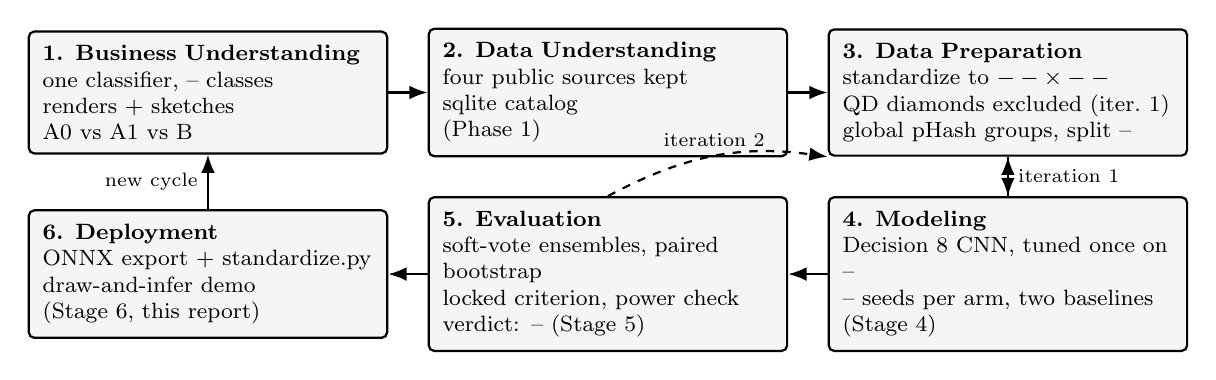
\begin{tikzpicture}[
  node distance=5mm,
  box/.style={draw, thick, rounded corners=2pt, fill=gray!8,
              font=\footnotesize, align=left, inner sep=5pt, text width=4.2cm},
  arr/.style={-Latex, thick},
]
\node[box] (bu) {\textbf{1. Business Understanding}\\ one classifier, \NumClasses{} classes\\ renders + sketches\\ A0 vs A1 vs B};
\node[box, right=of bu] (du) {\textbf{2. Data Understanding}\\ four public sources kept\\ sqlite catalog\\ (Phase 1)};
\node[box, right=of du] (dp) {\textbf{3. Data Preparation}\\ standardize to $\ImageSize{\times}\ImageSize$\\ QD diamonds excluded (iter.\ 1)\\ global pHash groups, split \SplitRatios{}};
\node[box, below=of dp] (mo) {\textbf{4. Modeling}\\ Decision 8 CNN, tuned once on \TuningArm\\ \SeedsPerArm{} seeds per arm, two baselines\\ (Stage 4)};
\node[box, left=of mo] (ev) {\textbf{5. Evaluation}\\ soft-vote ensembles, paired bootstrap\\ locked criterion, power check\\ verdict: \Verdict{} (Stage 5)};
\node[box, left=of ev] (de) {\textbf{6. Deployment}\\ ONNX export + standardize.py\\ draw-and-infer demo\\ (Stage 6, this report)};
\draw[arr] (bu) -- (du);
\draw[arr] (du) -- (dp);
\draw[arr] (dp) -- (mo);
\draw[arr] (mo) -- (ev);
\draw[arr] (ev) -- (de);
\draw[arr] (de.north) -- node[font=\scriptsize, left]{new cycle} (bu.south);
\draw[arr, dashed] (mo.north) -- node[font=\scriptsize, right]{iteration 1} (dp.south);
\draw[arr, dashed] (ev.north) to[bend left=18] node[font=\scriptsize, above]{iteration 2} (dp.south west);
\end{tikzpicture}}
\caption{The project on CRISP-DM. Every step is now covered; Deployment, left
open in Phase 1, is closed by the exported model and the demo (Section F). The
dashed arrow is iteration 1: a Modeling finding sent the project back to Data
Preparation (Section B, \emph{CRISP-DM iteration 1}). The second dashed arrow
is iteration 2: an Evaluation finding sent the project back to Data Preparation
(Section K).}
\label{fig:crisp}
\end{figure}

% =====================================================================
\section*{B. Data and splits}
\addcontentsline{toc}{section}{B. Data and splits}
% =====================================================================

\textbf{Sources.} Four public datasets, the same as in Phase 1: Quick, Draw!
\cite{quickdraw} (sketch), reevald's \emph{Geometric Shapes Mathematics}
\cite{kagglereevald} (render), El Korchi's 2D geometric shapes
\cite{elkorchi} (render; only source of pentagons) and the Hand-Drawn Shapes
dataset \cite{handdrawn} (sketch; only source of ellipses). Every image is
standardized to $\ImageSize{\times}\ImageSize$, single channel, black outline on
white.

\textbf{Split (Stage 1).} The data is split \SplitRatios{} into train,
validation and test by perceptual-hash near-duplicate group. Following
Decision 15, groups are now formed \emph{globally over all sources}
(Hamming distance at most \PhashHammingMax{} bits), so a shape two sources
drew near-identically can no longer straddle train and test. The Phase 1
counts are therefore not reproduced; the frozen split holds \SplitTrain{}
train, \SplitVal{} validation and \SplitTest{} test images
(\SplitTotal{} in total), in \NearDupGroups{} near-duplicate groups, the
largest of which has \LargestNearDupGroup{} images. The split files live in
Git (\nolinkurl{configs/splits/}) and are read only through
\nolinkurl{common.load_split}; this report never reads the test split.

\textbf{CRISP-DM iteration 1: Quick, Draw! diamonds excluded.} The plan
(Decision 1) was to remove only the gemstone drawings from Quick, Draw!'s
\texttt{diamond} class, using a reviewed md5 list. Inspecting the review
contact sheets (Figure~\ref{fig:qddiamonds}) showed a larger problem: most of
these drawings are not rhombi at all but gemstones, cones, shields, single
strokes and scribbles, which contradicts the taxonomy definition
(\emph{rhombus without right angles}). Models trained on the first data
freeze confirmed it on the \emph{validation} split (no test data was used,
Table~\ref{tab:iter1}): diamonds rendered by reevald were recognised well, but
recall on Quick, Draw! ``diamonds'' depended on whether a model memorised the
doodle style. The unaugmented A0 recalled most of them; the augmented A1,
which generalises the geometry, labelled many of the cone- and
shield-shaped ``diamonds'' as triangles (\IterOneAOneSeedZeroQDAsTriangle{} of
\IterOneAZeroSeedZeroQDN{} for seed 0). The label noise therefore
\emph{penalises} exactly the arms that learn the textbook shape, and arm B,
whose synthetic diamonds are true rhombi, most of all: it would have biased
the primary B vs A1 comparison. The project looped from Modeling back to Data
Preparation (Figure~\ref{fig:crisp}, dashed arrow): all Quick, Draw!
diamonds are excluded by a rule (configuration key
\texttt{exclude\_source\_labels}), \emph{before} the split, which removed
\ExcludedByRule{} drawings; the data were re-frozen and every model was
retrained from scratch. The per-image gemstone list is superseded (filter
state: \GemstoneFilterState). The evidence is kept in
\nolinkurl{docs/crisp_dm/}, generated from the validation outputs of the
first freeze.

\begin{table}[H]
\centering\footnotesize
\begin{tabular}{lrrrr}
\toprule
Run (first freeze) & macro-F1 & diamond F1 & recall, reevald rhombi & recall, Quick, Draw! ``diamonds'' \\
\midrule
A0, seed 0 & \IterOneAZeroSeedZeroMacroFone & \IterOneAZeroSeedZeroDiamondFone & \IterOneAZeroSeedZeroRenderRecall\% & \IterOneAZeroSeedZeroQDRecall\% \\
A0, seed 2 & \IterOneAZeroSeedTwoMacroFone & \IterOneAZeroSeedTwoDiamondFone & \IterOneAZeroSeedTwoRenderRecall\% & \IterOneAZeroSeedTwoQDRecall\% \\
A1, seed 0 & \IterOneAOneSeedZeroMacroFone & \IterOneAOneSeedZeroDiamondFone & \IterOneAOneSeedZeroRenderRecall\% & \IterOneAOneSeedZeroQDRecall\% \\
A1, seed 2 & \IterOneAOneSeedTwoMacroFone & \IterOneAOneSeedTwoDiamondFone & \IterOneAOneSeedTwoRenderRecall\% & \IterOneAOneSeedTwoQDRecall\% \\
\bottomrule
\end{tabular}
\caption{CRISP-DM iteration 1 evidence, validation split of the first data
freeze (generated: \nolinkurl{docs/crisp_dm/iteration_1_quickdraw_diamonds.json}).
Augmented models recognise rendered rhombi but reject many Quick, Draw!
``diamonds'', which are mostly not rhombi.}
\label{tab:iter1}
\end{table}

\begin{figure}[H]
\centering
\GuardedGraphic{0.8\linewidth}{figures/quickdraw_diamond_doodles.png}
\caption{One page of the Quick, Draw! \texttt{diamond} review sheet (image id
suffix and md5 prefix under each drawing). Few drawings are rhombi; most are
gemstones, cones, shields or scribbles.}
\label{fig:qddiamonds}
\end{figure}

\textbf{Source-shortcut check (Stage 1, Decision 12).} A source classifier
trained on standardized pixels of classes with two or more sources reached
\SourceClassifierAccPct\% pooled accuracy against a majority-source rate of
\SourceMajorityRatePct\% (gain \SourceGainPoints{} points; trigger
\ShortcutTriggerPoints{} points). Shortcut detected: \textbf{\ShortcutDetected}.
When it fires, the per-source table becomes mandatory, pentagon and ellipse
carry an asterisk, and a leave-one-source-out run is required
(leave-one-source-out required: \LosoRequired; held-out source:
\LosoHoldoutSource).

% =====================================================================
\section*{C. Methods}
\addcontentsline{toc}{section}{C. Methods}
% =====================================================================

\subsection*{C.1 Augmentation (Stage 2, arms A1 and B)}

Training images get rotation, uniform scale, translation, salt noise and
Gaussian blur, with the ranges in the \texttt{augment} section of
\nolinkurl{configs/pipeline.yaml}.
Two transforms would change the geometric class, so they are disabled for
the ambiguous classes listed in \nolinkurl{configs/taxonomy.yaml}: shear
and non-uniform scale never touch circle, ellipse, square, rectangle or
diamond (a sheared square is a diamond, a stretched circle is an ellipse).
Every output is re-thresholded, so an augmented image is still a clean
outline. Augmentation runs on the fly on the training stream only, after the
split, and is identical for A1 and B. Figure~\ref{fig:augqa} is the QA sheet
the stage renders for review.

\begin{figure}[H]
\centering
\GuardedGraphic{0.85\linewidth}{docs/crisp_dm/iteration_1/figures/qa_stage2.png}
\caption{Stage 2 QA sheet: one row per class, original followed by augmented
samples.}
\label{fig:augqa}
\end{figure}

\subsection*{C.2 Synthetic generator (Stage 3, arm B)}

The generator draws each class procedurally with Pillow at a supersampled
resolution, then downsamples and thresholds to the same
$\ImageSize{\times}\ImageSize$ outline format as the real data. Its parameter
ranges live in the \texttt{synth} section of \nolinkurl{configs/pipeline.yaml};
the ambiguity margins
in \nolinkurl{configs/taxonomy.yaml} keep every synthetic image clearly on
one side of the three ambiguous pairs (an ellipse's axis ratio and a
rectangle's side ratio stay above their minimum, a diamond's angle stays
away from a right angle). Table~\ref{tab:paramranges} lists the realized
ranges from \nolinkurl{artifacts/stage3/param_ranges.json} and the margins in
force. Throughput: \ThroughputSynth{} images per second against a target of
\ThroughputTarget.

\begin{table}[H]
\centering
\caption{Realized generator parameter ranges per class and the margins in
force (generated from \texttt{artifacts/stage3/param\_ranges.json}).}
\label{tab:paramranges}
\scriptsize
\InputIfFileExists{docs/crisp_dm/iteration_1/param_ranges.tex}{}{--}
\end{table}

\begin{figure}[H]
\centering
\GuardedGraphic{0.85\linewidth}{docs/crisp_dm/iteration_1/figures/qa_stage3.png}
\caption{Stage 3 QA sheet: synthetic samples per class.}
\label{fig:synthqa}
\end{figure}

\subsection*{C.3 Training (Stage 4)}

\textbf{Model (Decision 8).} A small CNN: input
$1{\times}\ImageSize{\times}\ImageSize$, four blocks of
[Conv $3{\times}3$ $\to$ BatchNorm $\to$ ReLU $\to$ MaxPool] with 32, 64, 128 and
128 channels, global average pooling, dropout and a linear layer to
\NumClasses{} logits. Training uses AdamW with a cosine schedule, batch size
\BatchSize, at most \MaxEpochs{} epochs and early stopping with patience
\Patience{} on validation macro-F1. All of this is read from the
\texttt{train} section of \nolinkurl{configs/pipeline.yaml}.

\textbf{Tuning (Decision 7).} Hyperparameters were tuned \emph{once}, on arm
\TuningArm's validation split, over the grid learning rate
$\{\TuningLRs\}$ $\times$ dropout $\{\TuningDropouts\}$ with one seed. The
winner (learning rate \TunedLR, dropout \TunedDropout) was frozen for every
arm and every seed; no arm was tuned separately.

\textbf{Step budget (Decision 13).} Because the loader uses class-balanced
sampling (Decision 11), an epoch is a fixed number of optimizer steps, not a
pass over the data. \texttt{steps\_per\_epoch} was computed once from arm A0
and frozen at \StepsPerEpoch; every arm runs the same steps per epoch, the
same maximum epochs and the same early-stopping rule. In arm B,
\SyntheticSharePct\% of each batch is synthetic, spread evenly across the
classes: \RealDrawsB{} real and \SynthDrawsB{} synthetic images per step,
against \RealDrawsA{} real images per step in A1.

\textbf{Seeds and runs.} Each arm is trained with \SeedsPerArm{} seeds
(\NumRuns{} CNN runs in total), identical settings everywhere. The seed
models of an arm are later combined into a soft-vote ensemble. The loader
benchmark measured \LoaderImagesPerSec{} images per second on the heaviest
stream (arm B).

\textbf{Baselines (Decision 14).} Logistic regression on raw pixels and a
linear SVM on HOG features train on the same class-balanced real stream as
A0 and are selected on validation. They are context, not part of the primary
hypothesis.

\subsection*{C.4 Evaluation protocol (Stage 5)}

\begin{itemize}
  \item \textbf{Power check first.} Before any test prediction, the paired
        bootstrap is run on A1's and B's \emph{validation} probabilities and
        the half-width rescaled by $\sqrt{n_{\mathrm{val}}/n_{\mathrm{test}}}$.
        If the expected half-width exceeds \PowerLimitPoints{} point, the
        report says so up front; the criterion is not changed
        (Table~\ref{tab:power}).
  \item \textbf{Test set read once per model.} Every seed model and both
        baselines are evaluated once on the locked test split and their
        probabilities cached; ensembles are formed from the cache. Stage 5 is
        the only stage allowed to read the test split, and the access log
        counts \TestReads{} reads for this run (Table~\ref{tab:testreads}).
  \item \textbf{Primary hypothesis (Decision 9).} B vs A1 on macro-F1 of the
        soft-vote ensembles, $\alpha = \Alpha$, paired bootstrap
        \CILevelPct\% CI with \NBoot{} resamples. McNemar's test on paired
        correctness is the supporting accuracy comparison. Per-seed paired
        differences (seed $k$ of A1 vs seed $k$ of B) are the robustness check.
  \item \textbf{Secondary comparisons.} A0 vs A1 and A0 vs B with a Holm
        correction across the two McNemar p-values.
  \item \textbf{Locked criterion (Decision 10).} B passes if the ensemble
        macro-F1 gain is at least \MinGainPoints{} point with a CI excluding
        zero, \emph{and} no class has both an F1 drop above its own threshold
        $\max(\MaxClassDropPoints, \text{noise band})$ and a paired bootstrap
        CI for that drop excluding zero. The noise band per class comes from
        \nolinkurl{artifacts/stage1/noise_bands.csv} (written by Stage 1 from
        the per-class test counts), because test classes are not equally
        sized. A drop inside the band is reported but does not
        fail the criterion. Per-class and per-source results are descriptive.
\end{itemize}

% =====================================================================
\section*{D. Results}
\addcontentsline{toc}{section}{D. Results}
% =====================================================================

Every table in this section is \texttt{\textbackslash input} from
\nolinkurl{docs/crisp_dm/iteration_1/tables/} exactly as Stage 5 wrote it; nothing is
retyped. If a table shows only a dash, Stage 5 has not run on this machine.

\textbf{What the primary number means (Decision 13).} B is compared with A1
at the \emph{same step budget} (\StepsPerEpoch{} steps per epoch, the same
maximum epochs, the same early stopping), with \SyntheticSharePct\% of each
batch \emph{substituted} by synthetic images rather than added: B draws
\RealDrawsB{} real images per step where A1 draws \RealDrawsA. Over the
frozen budget B therefore sees fewer real-image draws than A1. The
comparison is equal-compute, and the number answers ``does swapping in
synthetic data help?'', not ``does adding it help?''. The latter is the
deferred \texttt{B\_equalreal} ablation (Section H).

\textbf{Verdict.} \begingroup\catcode`\<=\active\def<{\textless{}}%
\InputIfFileExists{docs/crisp_dm/iteration_1/tables/verdict.tex}{}{--}\endgroup
\par\noindent Stage 5 status verdict: \textbf{\Verdict}. A failed verdict
with honest confidence intervals is a valid, reportable result: in CRISP-DM
terms the loop goes back to business understanding, and the likely levers are
the synthetic ratio, the generator or the label rules.

\begin{table}[H]
\centering
\caption{Accuracy (\%) and macro-F1 (points) on the locked test split: seed
models, per-seed mean $\pm$ std, soft-vote ensembles and baselines.}
\label{tab:metrics}
\small
\InputIfFileExists{docs/crisp_dm/iteration_1/tables/metrics.tex}{}{--}
\end{table}

\begin{table}[H]
\centering
\caption{Paired comparisons: the primary B vs A1 test and the two Holm-corrected
secondary tests, with per-seed robustness (mean $\pm$ std of the paired
per-seed differences and whether every seed has the same sign).}
\label{tab:comparisons}
\IfFileExists{docs/crisp_dm/iteration_1/tables/comparisons.tex}{\resizebox{\linewidth}{!}{\begin{tabular}{lrrrrrrrrr}
\toprule
comparison & role & delta\_macro\_f1\_points & ci & mcnemar\_b & mcnemar\_c & p\_raw & p\_holm & per\_seed\_mean\_std & same\_sign \\
\midrule
B vs A1 & primary & -0.4 & [-1.2, 0.4] & 53 & 44 & 0.417 & -- & 0.1 ± 1.0 & no \\
A1 vs A0 & secondary (Holm) & -3.0 & [-4.2, -1.8] & 158 & 77 & 0.000 & 0.000 & -1.6 ± 2.8 & no \\
B vs A0 & secondary (Holm) & -3.4 & [-4.5, -2.2] & 166 & 76 & 0.000 & 0.000 & -1.5 ± 2.4 & no \\
\bottomrule
\end{tabular}
}}{--}
\end{table}

\begin{table}[H]
\centering
\caption{Per-class ensemble F1 with the B $-$ A1 change, its lower CI bound,
the class threshold $\max(\MaxClassDropPoints, \text{noise band})$ and the
guardrail flag. An asterisk marks a single-source class when the Stage 1
shortcut check fired.}
\label{tab:perclass}
\IfFileExists{docs/crisp_dm/iteration_1/tables/per_class.tex}{\resizebox{\linewidth}{!}{\begin{tabular}{lrrrrrrrr}
\toprule
class & n\_test & f1\_A0 & f1\_A1 & f1\_B & drop\_B\_minus\_A1 & drop\_ci\_lo & threshold & flag \\
\midrule
circle & 375 & 95.7 & 95.2 & 95.1 & -0.1 & -1.2 & 2.0 &  \\
ellipse* & 149 & 84.4 & 82.8 & 80.7 & -2.0 & -1.4 & 2.5 & reported \\
triangle & 572 & 95.6 & 94.8 & 94.5 & -0.4 & -0.6 & 2.0 &  \\
square & 375 & 97.6 & 90.3 & 89.7 & -0.5 & -0.9 & 2.0 &  \\
rectangle & 301 & 93.3 & 80.2 & 79.3 & -0.9 & -1.6 & 2.0 &  \\
pentagon* & 157 & 99.0 & 99.7 & 99.0 & -0.6 & 0.0 & 2.4 &  \\
hexagon & 226 & 88.3 & 89.7 & 90.5 & +0.9 & -2.6 & 2.0 &  \\
octagon & 226 & 87.2 & 90.8 & 91.3 & +0.5 & -2.0 & 2.0 &  \\
star & 245 & 98.6 & 99.2 & 99.4 & +0.2 & -0.7 & 2.0 &  \\
diamond* & 150 & 99.0 & 86.0 & 85.4 & -0.7 & -2.9 & 2.4 &  \\
\bottomrule
\end{tabular}
}}{--}
\end{table}

\textbf{Same-source vs unseen-source generalization (R19).} The primary test
measures \emph{same-source} generalization: the test images come from the
same four sources as the training images, held out by pHash group. Rows
labelled ``unseen-source generalization'' in Table~\ref{tab:persource}, if
present, come from the leave-one-source-out runs (A1 and B retrained without
the Hand-Drawn source and tested on Hand-Drawn only; required: \LosoRequired).
Hand-Drawn is the only source of ellipses, so these runs train on nine classes
and are scored on Hand-Drawn triangles and rectangles only, the two other
classes that source contains; they say nothing about unseen-source ellipses.
Neither number is universal sketch generalization: the same-source result
says how the model does on more drawings from the sources it saw, the
unseen-source result says how it does on one specific source it never saw.

\begin{table}[H]
\centering
\caption{Ensemble accuracy per source and per domain (render vs sketch).
``Held-out source'' rows are the unseen-source leave-one-source-out results.}
\label{tab:persource}
\small
\InputIfFileExists{docs/crisp_dm/iteration_1/tables/per_source.tex}{}{--}
\end{table}

\textbf{Seed robustness.} Mean pairwise disagreement between seed models on
validation: A0 \SeedDisagreementAzero\%, A1 \SeedDisagreementAone\%,
B \SeedDisagreementB\%. This is a robustness number, not the power estimate:
the primary CI resamples test images, not seeds.

\begin{table}[H]
\centering
\caption{Power check, run on validation before the test set was opened.}
\label{tab:power}
\small
\InputIfFileExists{docs/crisp_dm/iteration_1/tables/power.tex}{}{--}
\end{table}

\begin{table}[H]
\centering
\caption{Test-split access accounting for this run (one read per trained model
and per baseline).}
\label{tab:testreads}
\small
\InputIfFileExists{docs/crisp_dm/iteration_1/tables/test_reads.tex}{}{--}
\end{table}

\begin{figure}[H]
\centering
\GuardedGraphic{0.32\linewidth}{docs/crisp_dm/iteration_1/figures/confusion_A0.png}\hfill
\GuardedGraphic{0.32\linewidth}{docs/crisp_dm/iteration_1/figures/confusion_A1.png}\hfill
\GuardedGraphic{0.32\linewidth}{docs/crisp_dm/iteration_1/figures/confusion_B.png}
\caption{Confusion matrices of the soft-vote ensembles on the test split:
A0 (left), A1 (middle), B (right).}
\label{fig:confusion}
\end{figure}

\begin{figure}[H]
\centering
\GuardedGraphic{0.68\linewidth}{docs/crisp_dm/iteration_1/figures/errors_square_diamond.png}\\[4pt]
\GuardedGraphic{0.68\linewidth}{docs/crisp_dm/iteration_1/figures/errors_square_rectangle.png}\\[4pt]
\GuardedGraphic{0.68\linewidth}{docs/crisp_dm/iteration_1/figures/errors_circle_ellipse.png}
\caption{Error galleries for the three ambiguous pairs (square/diamond,
square/rectangle, circle/ellipse), rendered by Stage 5. Stage 6 may not read
test images, so these are shown exactly as written.}
\label{fig:errors}
\end{figure}

% =====================================================================
\section*{E. Limitations}
\addcontentsline{toc}{section}{E. Limitations}
% =====================================================================

\begin{itemize}
  \item \textbf{reevald's dashed outlines.} The fill-to-outline filter removes
        the fill cue, but reevald's dashed strokes are kept as drawn and still
        hint at the source. Table~\ref{tab:persource} shows whether that
        source behaves differently.
  \item \textbf{Diamond is now render-only.} CRISP-DM iteration 1 removed all
        Quick, Draw! diamonds (\ExcludedByRule{} drawings) because most were
        not rhombi. The diamond class now comes from reevald's renders only,
        like pentagon (El Korchi) and ellipse (Hand-Drawn) it is a
        single-source class, and the model has seen no sketched diamond;
        sketched rhombi in the demo are out of its training distribution.
  \item \textbf{Near-duplicate pentagons.} El Korchi shapes differ mostly in
        colour, size and position, which standardization removes, so they
        collapse into large near-duplicate groups (the largest holds
        \LargestNearDupGroup{} images). A group is assigned whole, so the
        pentagon class can sit off the \SplitRatios{} targets and its test
        images are less diverse than their count suggests.
  \item \textbf{Single-source classes.} Pentagon comes only from El Korchi and
        ellipse only from Hand-Drawn. For these classes ``which shape'' and
        ``which source'' cannot be separated. The Stage 1 source-classifier
        check (shortcut detected: \ShortcutDetected) says how strong the source
        cue is in the shared classes; when it fired, the per-class table stars
        both classes and the leave-one-source-out result is the honest
        complement. Because Hand-Drawn owns the ellipse class, that complement
        covers nine trained classes and two scored ones, not the full task.
  \item \textbf{Equal-compute framing.} The primary number compares
        substitution, not addition, of synthetic data (Section D). A
        different framing (\texttt{B\_equalreal}) could give a different
        answer and was deferred (Section H).
  \item \textbf{Compute budget.} Training ran on one GPU with \SeedsPerArm{} seeds
        per arm and a small CNN. The seed-robustness numbers above bound how
        much the per-seed results move; more seeds would narrow them but not
        the primary CI, which is driven by the test-set size.
  \item \textbf{Demo evidence is informal.} Drawings made in the demo are not
        test data and never change the verdict (Section F).
\end{itemize}

% =====================================================================
\section*{F. Deployment (CRISP-DM step 6)}
\addcontentsline{toc}{section}{F. Deployment}
% =====================================================================

\textbf{Export bundle.} Stage 6 exports the run with the best
\emph{validation} macro-F1 (\ExportedRun, arm \ExportedArm, validation
macro-F1 \ExportedValFone{} as recorded in \nolinkurl{export/model_card.json};
the test split never enters the choice) to \nolinkurl{export/} as
\nolinkurl{model.onnx}, together with a verbatim copy of the training
\nolinkurl{standardize.py}, \nolinkurl{predict.py} and \nolinkurl{labels.json}.
The bundle imports nothing from the project. A smoke test in the pipeline
loads it in a fresh interpreter and predicts a procedurally drawn hexagon of
arbitrary size; its result is in \nolinkurl{artifacts/stage6/status.json}.

\textbf{Draw-and-infer demo.} \texttt{python run\_pipeline.py --demo} opens a
Gradio page with a $256{\times}256$ canvas (black 8 px stroke on white),
an \textbf{Infer} and a \textbf{Clear} button. Infer sends the
drawing through \nolinkurl{export/predict.py}, which calls the same
\nolinkurl{standardize.py} used in training, so there is no train/serve skew,
and shows the predicted class, the top-3 confidences and the
$\ImageSize{\times}\ImageSize$ image the model actually saw. Edge cases: an
empty canvas (tested on the alpha channel) or a contrast-free mark shows
``Draw a shape first''; a top confidence below 0.5 is shown as ``not sure'';
a missing model shows ``no exported model yet''.

\textbf{Demo drawings are informal evidence only.} They are not test data,
are never used for training and never change the verdict; the live sketch
check the team runs with the demo is an anecdote, not a result.

% =====================================================================
\section*{G. Reproducibility}
\addcontentsline{toc}{section}{G. Reproducibility}
% =====================================================================

The Stage 5 run that produced the results above has run id \texttt{\RunId}
and read the test split \TestReads{} times (Table~\ref{tab:testreads}). Every
stage records the hashes of its inputs in \nolinkurl{artifacts/stageN/status.json}
and is skipped when they match. To rebuild everything from the frozen split:
\texttt{python run\_pipeline.py} (all stages), or
\texttt{python run\_pipeline.py --stages 6} to regenerate the export, this
report and its traceability check only. The report is compiled with
\texttt{.\textbackslash build.ps1 -File phase2\_report.tex}; the dashboard
(\texttt{--dashboard}) shows every stage's status.

\textbf{Reproducibility of training.} Every CNN, including the tuning grid, was
trained on one GPU with one software build. The device, GPU model and torch
build are part of each run's recipe fingerprint, so a run is reused only on
identical hardware. Retraining the whole sweep after an unrelated code fix gave
validation probabilities identical to the bit for every run, so training is
deterministic on this setup; other hardware can give different numbers.

% =====================================================================
\section*{H. Ablations (deferred)}
\addcontentsline{toc}{section}{H. Ablations (deferred)}
% =====================================================================

The plan lists ablations as ``if time allows''. None were run for this
report; each is a new entry in the \texttt{runs} list of
\nolinkurl{configs/pipeline.yaml} and the pipeline would train and evaluate it
with no code change:
\begin{itemize}
  \item \texttt{B\_equalreal} (Decision 13): \BatchSize{} real images plus the
        synthetic share added on top, same step budget, so synthetic data is
        \emph{added} rather than substituted.
  \item Synthetic ratio 0/15/30/50\% (the 0\% point is A1 and is already
        available).
  \item Per-augmentation removal (rotation, scale, translation, noise, blur).
  \item A sketch-only test slice (Quick, Draw! and Hand-Drawn images only).
\end{itemize}

% =====================================================================
\section*{I. Course requirements checklist}
\addcontentsline{toc}{section}{I. Course requirements checklist}
% =====================================================================

The official Phase 2 rubric and page/format limits were not available in the
repository when this report was built. The checklist below lists every item
the plan expects the rubric to contain; each is marked pending until the team
fills it from the official document, and any unmet item is a submission
blocker. No requirement has been invented here.

\begin{table}[H]
\centering
\caption{Rubric checklist (implementation.md, Course requirements checklist).}
\label{tab:rubric}
\small
\begin{tabularx}{\linewidth}{@{}>{\raggedright\arraybackslash}p{5.2cm} >{\raggedright\arraybackslash}X p{4.6cm}@{}}
\toprule
Rubric item & What this submission provides & Status \\
\midrule
Deadline and submission channel & -- & \pending \\
Required sections and page/file limits & Sections A--J of this report & \pending \\
Required model families or baselines & CNN (three arms) plus logistic regression and linear SVM baselines & \pending \\
Required validation/statistical methods & paired bootstrap CI, McNemar, Holm correction, power check, locked criterion & \pending \\
Required data/FD/CRISP-DM evidence carried from Phase 1 & Phase 1 report; CRISP-DM recap in Section A & \pending \\
Required demo, export, reproducibility or individual-contribution evidence & export bundle, demo, status files, run id (Sections F--G); contribution record pending & \pending \\
Citation and file-naming rules & bibliography below & \pending \\
\bottomrule
\end{tabularx}
\end{table}

% =====================================================================
\section*{J. Data and model credits, redistribution}
\addcontentsline{toc}{section}{J. Data and model credits, redistribution}
% =====================================================================

\textbf{Training data.} The model was trained on images from four public
sources: Quick, Draw! by Google Creative Lab \cite{quickdraw} (CC BY 4.0),
\emph{Geometric Shapes Mathematics} by reevald on Kaggle \cite{kagglereevald}
(CC0, public domain), the \emph{2D geometric shapes dataset} by A. El Korchi
on Mendeley Data \cite{elkorchi} (CC BY 4.0) and the \emph{Hand-Drawn Shapes
Dataset} by frobertpixto on GitHub \cite{handdrawn} (CC BY 4.0 for the data,
MIT for its code). Links and license statements are in the bibliography.
Preparation applied to all of them: standardization to
$\ImageSize{\times}\ImageSize$ outlines, the rule-based exclusion of all Quick, Draw!
diamonds (CRISP-DM iteration 1; gemstone list state:
\GemstoneFilterState), exact and near-duplicate grouping, and the
\SplitRatios{} group split. The same notice is in
\nolinkurl{export/README.md}, and the demo links to it under ``Data and model
credits''.

\textbf{What is redistributed.} The export bundle contains model weights
(\nolinkurl{model.onnx}) and code (\nolinkurl{predict.py},
\nolinkurl{standardize.py}, the export and demo code). It contains no training
images and no derived outlines. The license for the team's own code and model
weights is a team decision that has not been made yet; until it is, the bundle
is not licensed for reuse, and the source-dataset licenses above apply to the
data they cover.

\newpage
% =====================================================================
% =====================================================================
\section*{K. CRISP-DM iteration 2}
\addcontentsline{toc}{section}{K. CRISP-DM iteration 2}
% =====================================================================

Iteration 1 ended with a valid fail: synthetic data did not improve on
augmentation, and the unaugmented arm scored highest. Finding a problem at
Evaluation and going back is part of the CRISP-DM loop. An investigation on
train and validation data only then looked for the cause, before any new
training. The iteration 1 verdict in Section D stands and is not rewritten.

\textbf{Findings at each step.}

{\small\InputIfFileExists{artifacts/stage6/generated/iteration_log.tex}{}{--}}

\textbf{Failures and how each was handled, in the order they happened.} Some were fixed, and some remain open.

{\small\InputIfFileExists{artifacts/stage6/generated/failures.tex}{}{--}}

\textbf{Changes and review points by CRISP-DM step.} Every change to data,
training or evaluation is filed under its step, followed by what two outside
code reviews raised after iteration 2 closed. No verdict changed as a result.

{\small\InputIfFileExists{artifacts/stage6/generated/changes.tex}{}{--}}

\textbf{What changed.} The transform defects were fixed, then the augmentation
and generator settings were tuned on validation only, under a plan committed
before tuning (\nolinkurl{docs/crisp_dm/iteration_2/preregistration.md}). A new
arm, \textbf{A2}, mixes clean real, augmented real and synthetic images in each
batch: \ItwoAtwoClean\% clean and \ItwoAtwoSynth\% synthetic. Every arm got its
own learning-rate and dropout tuning. The search chose rotation of
$\pm$\ItwoRotate$^\circ$, capped at $\pm$\ItwoRotateCap$^\circ$ for square,
rectangle and diamond, and \ItwoBSynth\% synthetic images for B. Trials per arm:
A0 \ItwoTrialsAzero, A1 \ItwoTrialsAone, B \ItwoTrialsB, A2 \ItwoTrialsAtwo.
A0 has no augmentation settings to search, so it received fewer trials, which
gives the tuned arms some selection advantage on validation.

\begin{table}[H]
\centering
\caption{Iteration 2 macro-F1 by arm: mean on validation over the tuning seeds,
soft-vote ensemble on the reused test split, and on the fresh holdout.}
\label{tab:itertwo}
\begin{tabular}{lrrr}
\toprule
Arm & Validation & Reused test split & Fresh holdout \\
\midrule
A0 & \ItwoValAzero & \ItwoEnsAzero & \ItwoFreshAzero \\
A1 & \ItwoValAone & \ItwoEnsAone & \ItwoFreshAone \\
B & \ItwoValB & \ItwoEnsB & \ItwoFreshB \\
A2 & \ItwoValAtwo & \ItwoEnsAtwo & \ItwoFreshAtwo \\
\bottomrule
\end{tabular}
\end{table}

\textbf{Pre-registered result (\ItwoPrimary).} On the reused test split the
macro-F1 change is \ItwoDelta{} points, \CILevelPct\% paired bootstrap CI
[\ItwoCILo, \ItwoCIHi], verdict: \textbf{\ItwoVerdict}. On the fresh holdout of
\ItwoFreshN{} images the change is \ItwoFreshDelta{} points, CI
[\ItwoFreshCILo, \ItwoFreshCIHi], verdict: \textbf{\ItwoFreshVerdict}.

\textbf{How much weight this can carry.} The test split was read in iteration 1
and its per-class results shaped this plan, so a second read is weaker evidence
than a first. The fresh holdout has never informed any choice and is the cleaner
check, with limits: its images come from sources seen in training, and it holds
no Quick, Draw! sketches because every local drawing was already in the catalog.
It was read once per model, in this run only.

\textbf{Unseen source.} Mean accuracy of the Hand-Drawn hold-out models on
Hand-Drawn triangles and rectangles of the test split, three seeds per arm:
A0 \ItwoLosoAzero\%, A1 \ItwoLosoAone\%, B \ItwoLosoB\%, A2 \ItwoLosoAtwo\%.
Ellipse is excluded because Hand-Drawn is its only source.

\textbf{Limitations.} Rotation was tuned on validation, so the chosen range
favours whatever the same-source split rewards. Whether orientation is a cue
the deployed model may use is a design decision for the project owner.

\begin{table}[H]
\centering
\caption{Iteration 2 comparisons on the reused test split.}
\small
\IfFileExists{artifacts/stage5/tables/comparisons.tex}{\resizebox{\linewidth}{!}{\input{artifacts/stage5/tables/comparisons.tex}}}{--}
\end{table}

\begin{table}[H]
\centering
\caption{Iteration 2 per-class F1 on the fresh holdout.}
\small
\InputIfFileExists{artifacts/stage5/tables/fresh_per_class.tex}{}{--}
\end{table}

\begin{thebibliography}{9}
\bibitem{quickdraw} Google Creative Lab. \emph{The Quick, Draw! Dataset}.
  License: CC BY 4.0.
  \url{https://github.com/googlecreativelab/quickdraw-dataset}
\bibitem{kagglereevald} reevald. \emph{Geometric Shapes Mathematics}.
  Kaggle. License: CC0, public domain.
  \url{https://www.kaggle.com/datasets/reevald/geometric-shapes-mathematics}
\bibitem{elkorchi} A. El Korchi. \emph{2D geometric shapes dataset}.
  Mendeley Data, DOI 10.17632/wzr2yv7r53.1. License: CC BY 4.0.
  \url{https://data.mendeley.com/datasets/wzr2yv7r53/1}
\bibitem{handdrawn} frobertpixto. \emph{Hand-Drawn Shapes Dataset}.
  GitHub. License: CC BY 4.0 (data), MIT (code).
  \url{https://github.com/frobertpixto/hand-drawn-shapes-dataset}
\bibitem{zauner} C. Zauner. \emph{Implementation and Benchmarking of
  Perceptual Image Hash Functions}. Master's thesis, 2010.
  \url{https://phash.org/docs/pubs/thesis_zauner.pdf}
\bibitem{lones} M. A. Lones. \emph{How to avoid machine learning
  pitfalls: a guide for academic researchers}. arXiv:2108.02497.
  \url{https://arxiv.org/abs/2108.02497}
\bibitem{lecdp} E. Mansour. COMP 333 lecture \emph{Introduction to Data
  Analysis: Data Preparation} (W4\_DP\_P1.pdf).
\bibitem{lecclf} E. Mansour. COMP 333 lecture \emph{Introduction to Data
  Analysis: Machine learning, classification}
  (week-6-lecture-3-classification.pdf).
\end{thebibliography}

\end{document}
